\chapter{Model Predictive Control}
\label{chap:Model_Predictive_Control}

\section{Introduction}

In this section the basic mathematical concepts required to understand the quadratic problem that arises in each iteration of Model Predictive Control will be briefly explained.

\subsection{Optimization problem}%------------------------------------------------------------------------------------------------------------------------------------------------------------------------------------------------------------

An optimization problem consists of finding a solution within a feasible set that minimizes or maximizes a performance index. These can be subdivided in continuous and discrete, depending on the nature of the variables. The standard mathematical formulation is described as follows:

\begin{equation} \label{eq:gen_qp}
 \begin{aligned}
 & \underset{x}{\text{minimize}}
 & V(x) \\
 & \text{subject to}
 & & f_i(x) \leq b_i, \; 	i = 1, \ldots, m.\\
 & & h_i(x) = b_i, \; 	i = 1, \ldots, n.\\
 \end{aligned}
\end{equation}

There are three elements to identify in this structure: the cost function $V(x)$, the equality constraints and the inequality constraints. Depending on the definition of the cost function and the constraints, the problem can be linear or quadratic, which are the most common types encountered in real life applications. 

\subsection{Quadratic programming problem}%-------------------------------------------------------------------------------------------------------------------------------------------------------------------------------------

A quadratic programming problem is a special case of an optimization problem where the cost function is a quadratic function and the constraints are linear. Given the variable  and gradient vector correspondingly $\mathbf{x}, \mathbf{g} \in \mathbb{R}^{n}$, both column vectors and Q a symmetric matrix of size $n \times n$, the quadratic problem can be formulated as follows: 

\begin{equation} \label{eq:quadproblem}
 \begin{aligned}
 & \underset{x}{\text{minimize}}
 & & V(x) = \frac{1}{2} \mathbf{x}^T Q \mathbf{x} + \mathbf{x}^T g \\
 & \text{subject to} 
 & & A\mathbf{x} \geq \mathbf b \mbox{  (inequality constraint)}
 \end{aligned}
\end{equation}

Where A is a matrix that represents the group of constraints and it is of size $m x n$, $b$ is a column vector of size $m$ that contains the limits in the constraints, where $m$ is the number of constraints. Equality constraints can be arranged into the $A$ and $b$ matrices with some manipulation.

\subsection{Active and Inactive Constraints and Sets}%----------------------------------------------------------------------------------------------------------------------------------------------------------------------

Given an optimization problem such as \ref{eq:gen_qp}, an inequality constraint $F_{i}(x) \leq b_{i}$ can be defined as \emph{active} at a point \~{x} in the feasible set when $F_{i} $(\~{x})$ = b_{i}$, and \emph{inactive} otherwise. Equality constraints are active in all its solutions that are as well contained in the region of the allowed possible solutions.\\

Therefore one can define the \emph{active set} at a point \~{x} as the combination of the region that satisfy the equality constraints and inequality constrains that become active at \~{x}. Correspondingly, The region that doesn't satisfy these conditions is called the \emph{inactive set}.

\subsection{Feasibility}%-------------------------------------------------------------------------------------------------------------------------------------------------------------------------------------------------------------------

When constraints are included in an optimization problem, they define the region where the possible solution exists. The resultant region is defined as the \emph{feasible} set.  The algorithms used to solve the problem require an initial point,  which depending on the specific application may be contained in the feasible set or not. The feasibility problem therefore consists in finding a feasible solution (if existent) regardless of the objective function.

\subsection{Convexity}%---------------------------------------------------------------------------------------------------------------------------------------------------------------------------------------------------------------------

A set of points $S \in \mathbb{R}^{n}$ is a convex set if the straight line connecting any two points that belong to S lies completely inside S. In a more formal definition, for any two points $x,y \in S$, the following is true $\alpha x + (1 - \alpha)y \in S, \forall \alpha \in [0,1]$. \\

This property is important because if this holds, the assumptions made for linear programming can be extended to cover convex optimization problems, and therefore be solved with fast and reliable methods that already exist for solving linear optimization problems.

\subsection{Karush-Kuhn-Tucker Conditions}%-------------------------------------------------------------------------------------------------------------------------------------------------------------------------------------------

The Karush-Kuhn-Tucker conditions (also knowns as KKT conditions) are a set of first order conditions that must be satisfied by the solution of nonlinear programming problems in general. It is formulated as an extension of the Lagrange multipliers method to solve optimization problems with equality constraints, as the KKT conditions applies for problems with constraints formulated as equalities and inequalities. These conditions are seldom used to solve directly the optimization problem, instead, they are verified in iterative methods. Before introducing the formal definition of the Karush-Kuhn-Tucker conditions, it is necessary to first define the Lagrangian for an optimization problem.\\

For the given form of the optimization problem shown in \ref{eq:gen_qp}, the Lagrangian $\mathbf{L}$ is defined as the cost function plus penalty functions that take into account the constraints. The $\lambda$ vector is used for the equality constraints and the $\mu$ vector for the inequalities.

\begin{equation} \label{eq:lagrangian}
\mathbf{L}(\mathbf{x}, \lambda, \mu) = f(x) + \sum \limits_{i=1}^{m} \lambda_{i} h_{i}(\mathbf{x}) + \sum \limits_{i=1}^{n} \mu_{i} f_{i}(\mathbf{x})
\end{equation}

If $x^{*}$ is a solution of \ref{eq:gen_qp} that satisfies some regularity conditions, then there are vectors $\lambda^{*}$ and $\mu^{*}$  such that the following conditions are satisfied:

\begin{itemize}
\item{Stationarity} \\

 & $\text{Minimization} && \nabla_{x} f(\mathbf{x}) + \sum  \limits_{i=1}^{m} \nabla_{x} \lambda_{i} h_{i}(\mathbf{x}) + \sum \limits_{i=1}^{n} \nabla_{x} \mu_{i} f_{i}(\mathbf{x}) = 0$\\

 & $\text{Maximization} && \nabla_{x} f(\mathbf{x}) + \sum  \limits_{i=1}^{m} \nabla_{x} \lambda_{i} h_{i}(\mathbf{x}) - \sum \limits_{i=1}^{n} \nabla_{x} \mu_{i} f_{i}(\mathbf{x}) = 0$\\

\item{Equality constraints} \\

 & $\nabla_{\lambda} f(\mathbf{x}) + \sum  \limits_{i=1}^{m} \nabla_{\lambda} \lambda_{i} h_{i}(\mathbf{x}) + \sum \limits_{i=1}^{n} \nabla_{\lambda} \mu_{i} f_{i}(\mathbf{x}) = 0$\\

\item{Complementary slackness condition}\\

 & $\mu_{i} f_{i}(\mathbf{x}) = 0, \forall i = 1, \ldots, n$\\

 &$\mu_{i} \geq 0, \forall i = 1, \ldots, n$\\

\end{itemize}

The stationarity conditions come from the derivation of the cost function to find the stationary points used in basic unconstrained optimization problems. The derivatives respect to the $\lambda$ coefficients (Lagrange multipliers) of the cost function lead to equations that restrict the solution of the problem to satisfy the equality constraints. However, due to the fact that the lagrangian also depends on $\mu$, the system is not determined. The complementary slackness conditions arises from the fact that if the optimal solution $x^{*}$ satisfies $f(\mathbf{x}) \leq 0$, its contribution to the cost function is null, and one can set its corresponding $\mu_{i}$ coefficient to cero. If the solution is at the border of the constraint,  $f(\mathbf{x}) = 0$. In both cases, the condition $\mu_{i} f_{i}(\mathbf{x}) = 0$ holds. The $\mu_{i}$ coefficients can take any value, but they are 0 when $f(\mathbf{x}) \leq 0$, and in the other case, $f(\mathbf{x}) = 0$, they can only be positive, since the gradient respect to $x$ of $f_{i}(\mathbf{x})$ and $V(\mathbf{x})$ are opposed in direction.\\

In the particular case of a quadratic programming problem as the ones that arise in Model Predictive Control, the problem becomes a convex optimization problem when the cost function is convex. A convex quadratic cost function is the one where the Hessian matrix $Q$ from \ref{eq:quadproblem} is positive semi-definite, the inequality constraints are convex functions and the equality constraints are linear. In the case of a convex quadratic programming program, the KKT conditions not only are necessary but also sufficient conditions for optimality.

\section{Model Predictive Control Theory} %------------------Model Predictive Control Basics---------------------------------------------

Model Predictive Control (MPC) is an advanced control technique developed in the late 70’s within the chemical industry. The basic idea in this algorithm is to use a model of the process or system to be controlled in order to predict and optimize future process behaviour. MPC can take into account restrictions in the input variables as well as the states/controlled variables \cite{Hovd2004}. This leads to solving an optimization problem in each sample, which demands high computing power in order to achieve this for small sampling times and deterministic operation.\\ 

There are several types of MPC controllers, but the basic steps of the algorithm are kept in each one of them, summarized as follows:

\begin{itemize}

\item Prediction: at each time instant, the model is used to get the predicted outputs of the process for as many time instants in the future as the prediction horizon states. These predictions depend on the past inputs and outputs and the future control signals to the model.

\item Optimization: the future control signals are calculated by either minimizing a cost index or maximizing a performance index that takes into account the error between the predicted outputs and the reference trajectory (or an approximation to it) and the control effort. This objective function to be optimized is usually a quadratic function, since it assures global minimum or maximum values, smoother control signals and more intuitive response to parameter changes \cite{Hovd2004}.

\item Shifting: the control signal for the current time instant $t$ is sent to the system and the next control signals in the future are rejected, since the output in the instant $t + 1$ is already known, and the prediction step is repeated with this new value and the information is brought to the following time step. Then the control signal corresponding to time instant    $t + 1$ will be calculated at time $t + 1$ (which is different from calculating the control signal for time $t + 1$ at time $t$, due to the new information).

\end{itemize}

\begin{figure}[h!]
\centering
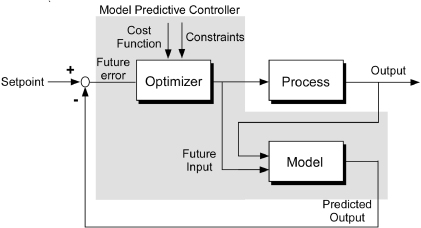
\includegraphics[scale=0.8]{Images/Chapter2/mpc_block_diagram.jpg}
\caption{Block diagram of the basic elements in Model Predictive Control \cite{Al-Sanad2005}.}
\label{fig:mpc_diagram}
\end{figure}

MPC controllers have some advantages compared to other control techniques, like the ones stated below:

\begin{itemize}

\item It can be used to control a great variety of processes, including ones that have long delay times or non-minimum phase or even unstable ones. 

\item In particular versions of MPC, it can be tuned to compensate for dead times.

\item The strategy is easily extendable to the multivariable case.

\item It can explicitly include constraints either on the control signal or the states/controlled variables.

\item It introduces feed forward in a natural way to compensate for measurable disturbances.

\end{itemize}

However, due to the characteristics of the technique, some drawbacks also arise:

\begin{itemize}

\item The main disadvantage to mention about MPC is the computing power required to solve the optimization problem in a suitable amount of time on each sampling instant, specially when the controlled systems have very fast dynamics. When the size of the problem is small, this can be solved by calculating all the possible control laws offline and then perform the look-up at runtime. However, the size of the optimization problem is also depending on the prediction horizon, which is a variable parameter considered for the tuning of the controller. This makes computational power an important aspect to consider in the implementation of MPC. Nowadays industrial computers shouldn't have problems hanlding this kind of processing, but since these are also used for several other functions, deterministic operation is important to preserve.

\item Another disadvantage of MPC is that the technique is dependant on the process model. The algorithm itself is independent of the model, but the quality of the control signal obtained through the optimization problem is strongly dependant on good predictions coming from the model. However, the integration of statistical methods of learning in recent works \cite{Bouffard2012} has been proven to solve this problem, without further modeling work.

\end{itemize}

\subsection{Model}%----------------------------------------Model--------------------------------------------------------------------------

Being of such importance to the performance of MPC controllers, the process model should be precise enough to capture all the important dynamics but simple enough to keep the optimization problem at a decent size, thus saving computational time when solving. Since MPC is not a unique strategy, different implementations of it may vary in the type of models used. However most implementations of MPC make use of one of these types of models: Transient Response, Transfer Function or State Space models. A brief description of each is presented in this section.

\begin{itemize}

\item \textbf{Transient Response.} Due to its simplicity, it is probably the most used kind of model in industry. To derive this kind of model, known inputs are fed to the real system or process and the outputs are measured. The most common inputs used for these experiments are impulse and step inputs, so in each corresponding case they are better known as impulse and step response models. The inputs and outputs are related by the following truncated sum of $N$ terms:

\begin{equation} \label{impulsemodel1}
y(k) = \sum_{i=1}^N h_i u(k-i) = H(z^{-1})u(k)
\end{equation}

where $H(z^{-1})$ is a polynomial of the backward shift operator, $z^{-1}$. For a model coming from such a simple experiment, the information that can be obtained is of great help to the understanding of the system: influenced variables by the input, time constants of the system and general characteristics can be determined from transient models. The fact that no previous knowledge of the system is required is an advantage for unknown processes. As a drawback, usually a lot of parameters are required as $N$ is usually a big number for these models.

\item \textbf{Transfer Function.} The transfer function model is obtained through the quotient of the Laplace transforms of the inputs and the outputs. When expressed in discrete time, these polynomials are a function of the backward shift operator, as stated below:

\begin{equation} \label{transferfunctionmodel1}
y(k) = \frac{B(z^{-1})}{A(z^{-1})}u(k)
\end{equation}

These models give a good physical insight and the resultant controller is of a low order and compact. However, to develop a good transfer function model some information of the system is required beforehand, more specifically about the order of the polynomials. Also, it is best suited for SISO systems.

\item \textbf{State Space.} The states of the system are described as a linear combination of the previous states and the inputs, and the output as a mapping of the states. The general form of state space models is as follows:

\begin{equation} \label{statespacemodel1}
\begin{cases} x(k + 1) = Ax(k) + Bu(k) \\ y(k) = Cx(k)
\end{cases}
\end{equation}

Where $A$ is the system matrix, $B$ is the input matrix and $C$ is the output matrix. The big advantage of this type of model is that it is straightforward to use for MIMO systems and the control law will always be a linear combination of the state vector. A drawback might be that the calculations could get complicated if a state observer is needed, as sometimes the state selection doesn't have any physical meaning.

\end{itemize}

For this thesis, the type of model used was the state space model representation. This selection allows an easier way to handle models of different sizes; also the recursive structure of the predictions from the model allows a more compact formulation of the quadratic problem, as developed by \cite{Ferreau2006}.


 
\subsection{Objective Function}%---------------------------Objective Function--------------------------------------------------------------

The objective function takes into account the error between reference trajectory and measured states, as well as the change in the control effort. The optimization process will give the values of the control signal $u$ that minimizes the values of this objective function. A basic form of this objective function would be the following:

\begin{equation} \label{objectivefunction1}
V(u) = \sum_{i=1}^{N_{p}}  [\hat{y}(k + i | k) - r(k + i)]^2 + \sum_{j=1}^{N_{c}} [\triangle u(k + i - 1)]^2
\end{equation}

Where the term $\hat{y}(k + i | k)$ represents the estimated output from the model calculated at time $k$ for any sample in the horizon, $r(k + i)$ is the reference trajectory desired for the process (which is usually known in applications such as robotics) and the term $\triangle u(k + i - 1)$ is the control effort. This objective function is quadratic, but it can also be linear or of a different order. Most MPC implementations use quadratic objective functions because they are independant on the sign of the optimised variable and they assure that a global minimum is reached. Some implementations of MPC use an approximation to the real reference trajectory which parameters can be tuned in order to adjust to fast tracking or smooth response.\\ 

Parameters $N_{p}$ and $N_{c}$ are the prediction and control horizon respectively. These can be set to the same number although it is not a necessary condition. The definition of these parameters define when it is of interest to consider the different errors. This allows the objective function to be flexible for systems with dead-times or non-minimum phase. Also these errors may have different relevance in the control of the system, therefore this objective function might include or not weight matrices in order to ponder differently the errors.\\

In this thesis, the objective function used is pre-defined by the optimization solver qpOASES, presented by \cite{Ferreau2006}, which is of the following form:

\begin{equation} \label{objectivefunction2}
V(u) = \frac{1}{2} \sum_{i=k_{0}}^{k_{0} + N_{p} - 1} (y_{k} - y_{ref})'Q(y_{k} - y_{ref}) + (u_{k} - u_{ref})'R(u_{k} - u_{ref}) + \frac{1}{2} (y_{k_{0} + n_{p}} - y_{ref})'P(y_{k_{0} + n_{p}} - y_{ref})
\end{equation}

In this equation, three sources of error are noticeable: output errors (or depending on the process, state errors), input errors and terminal cost errors. Each source has its respective weight matrix: Q, R and P, respectively. In this implementation, the prediction horizon and the control horizon have been merged into the same number $N_{p}$, simplifying the function.

\subsection{Constraints}%---------------------------------Constraints----------------------------------------------------------------------

Constraints are limitations in the values of the variables that are considered in the open loop optimization problem formulated in MPC. The explicit consideration of constraints is translated into an increase in computational complexity, as the solution of the problem can only be obtained through numerical methods. Usually, constraints in the inputs are due to limitations of the actuators interacting with the process, and constraints in the outputs or in the states come from safety or operational limits in the process itself or the sensors present in the system.\\

In \cite{Ferreau2006} a distinction is made between bounds and constraints, where the bounds are the limit values for the variable being optimised (the control signal $u$) and the constraints are expressions to define the limitations of the outputs and states, which are mapped through the matrix G as follows:

\begin{equation} \label{constraints1}
\underline{U} \leq u \leq \bar{U}
\end{equation}
\begin{equation} \label{constraints2}
\underline{A} \leq G\mathbf{x} \leq \bar{A} 
\end{equation}


\subsection{Optimization}%---------------------------Optimization--------------------------------------------------------------------------

There are two main type of algorithms used commonly to solve quadratic problems like the ones that arise in MPC: active set methods and interior point methods.

\begin{itemize}

\item \textbf{Active Set Methods.} 

%In order to explain how these methods work, a definition for an \emph{active set} must be introduced. An optimization problem:
 
%\begin{equation} \label{eq:optimization1}
% \begin{aligned}
% & \underset{x}{\text{minimize}}
 %& & V(x) \\
 %& \text{subject to}
 %& & f_i(x) \leq b_i, \; 	i = 1, \ldots, m.
 %\end{aligned}
%\end{equation}

%is defined by the objective function and by the set of constraints. This set defines the \emph{feasible region}, which is the set of all $x$ that satisfy the constraints, and thus are considered in the search for the optimal solution. Given $x$ in the feasible region, a constraint $f$ is active in $x$ if $f_i(x) = 0$ and inactive if $f_i(x) > 0$. The \emph{active set} at $x$ comprises all the constraints that are active at that point \cite{Nocedal&Wright2006}. \\

The aim of an Active Set method is to find an optimal active set, which will make it possible to use equality constrained QP solving techniques (solving the KKT system). The algorithm will start making a guess of this optimal active set, and if it misses, gradient and Lagrange multipliers will be used to improve the initial guess. The final solution of the problem will lie in the proximity of the borders of the  feasible region.

\item \textbf{Interior Point Methods.} Given the following quadratic problem in the standard form, shown in \ref{eq:quadproblem}, based on the KKT conditions one can say that if a given $x^*$ is a solution of \ref{eq:quadproblem}, there is a Lagrange multiplier vector $\lambda^*$ such that the following conditions are satisfied for $(x, \lambda) = (x^*, \lambda^*)$.

\begin{equation} \label{eq:KKTIP}
 \begin{subequations}
 \begin{aligned}
  Qx - A^{T}\lambda + g &= 0, \\
  Ax - b &\geq 0, \\ 
  (Ax - b)_{i}\lambda_{i} &= 0, && i = 1, 2, \ldots , m, \\
  \lambda &\geq 0. 
 \end{aligned}
 \end{subequations}
\end{equation}

If a new variable vector $y = Ax - b$ is introduced in the system, the conditions can be rewritten as follows.

\begin{equation} \label{eq:KKTIP2}
 \begin{subequations}
 \begin{aligned}
  Qx - A^{T}\lambda + g &= 0, \\
  Ax - y - b &= 0, \\ 
  y_{i}\lambda_{i} &= 0, && i = 1, 2, \ldots , m, \\
  (y, \lambda) &\geq 0. 
 \end{aligned}
 \end{subequations}
\end{equation}

Which are correspondent with the KKT conditions for linear programming problems \cite{Nocedal}. If we assume that we are only working with a convex objective function and feasible region, these conditions are necessary but also sufficient to assure the existence of such pair, and therefore the solution of the system \ref{eq:KKTIP2} solves the quadratic problem.

\end{itemize}

\subsection{Horizons}

In MPC, the horizons define how far is the controller making a prediction in the future. The typical horizons in MPC are the prediction horizon $N_p$, and the control horizon, $N_c$. The prediction horizon has the basic function described previously: defining the prediction lenght. The selection of $N_p$ is a matter of trial and error but it is highly dependant on the dynamics of the plant being considered. The prediction must be able to take into account the settling time of the system under a disturbance but also must be kept small enough so that it doesn't increase unneccessarily the size of the quadratic problem to solve. In order to have a better way to tune this, the control horizon $N_c$ tells the MPC how much solutions it must calculate, independently of the size of the prediction horizon, keeping the computations at the minimum.

\section{Summary}

In this chapter, the mathematical base for MPC has been described, in order to get a better understanding of the optimization problem ocurring at each step. Also, MPC is introduced, together with its basic steps and characteristics. The different elements in MPC are explained in separate items to cover the individual functions and importance of each within the algorithm.
